\documentclass[a4paper]{tufte-handout}

\title{The digimorse Communications Protocol}

\author{Matt Gumbley, M{\O}CUV}

%\date % without \date command, current date is supplied

%\geometry{showframe} % display margins for debugging page layout

\usepackage{graphicx} % allow embedded images
\setkeys{Gin}{width=\linewidth,totalheight=\textheight,keepaspectratio}
\graphicspath{{graphics/}} % set of paths to search for images
\usepackage{amsmath}  % extended mathematics
\usepackage{booktabs} % book-quality tables
\usepackage{units}    % non-stacked fractions and better unit spacing
\usepackage{multicol} % multiple column layout facilities
\usepackage{lipsum}   % filler text
\usepackage{fancyvrb} % extended verbatim environments
\usepackage{hyperref} % URLs
\fvset{fontsize=\normalsize}% default font size for fancy-verbatim environments

% Standardize command font styles and environments
\newcommand{\doccmd}[1]{\texttt{\textbackslash#1}}% command name -- adds backslash automatically
\newcommand{\docopt}[1]{\ensuremath{\langle}\textrm{\textit{#1}}\ensuremath{\rangle}}% optional command argument
\newcommand{\docarg}[1]{\textrm{\textit{#1}}}% (required) command argument
\newcommand{\docenv}[1]{\textsf{#1}}% environment name
\newcommand{\docpkg}[1]{\texttt{#1}}% package name
\newcommand{\doccls}[1]{\texttt{#1}}% document class name
\newcommand{\docclsopt}[1]{\texttt{#1}}% document class option name
\newenvironment{docspec}{\begin{quote}\noindent}{\end{quote}}% command specification environment

\begin{document}

    \maketitle% this prints the handout title, author, and date

    \begin{abstract}
        \noindent
        This document describes the rationale for, and the design of the digimorse communications protocol.
        It describes choices made at all stages of its implementation in the transceiver software.
    \end{abstract}

%\printclassoptions

    \newthought{The digimorse communications protocol exists} to bring together two aspects of amateur radio that I
    particularly
    enjoy, to see if the benefits of one aspect might improve my enjoyment of the other.
    Namely, to see if digital encoding and error correction\footnote{Such as found in the WSJT-X weak-signal mode
    software by Joe Taylor K1JT et al.} might be used to provide a significant coding gain, and a removal of noise
    from Morse Code - our historic mode of communication.

    Other features of modern digital operation that I aim to bring to Morse operation with digimorse include:
    \begin{itemize}
        \item a waterfall display
        \item active station information
        \item meaningful signal reports
    \end{itemize}

    Waterfall displays are now standard features on modern SDR\footnote{Software Defined Radio} transceivers such as
    the Yaesu FTDX10, and in software such as WSJT-X\cite{FT4FT8}.
    They show the presence of any signals across the receiver's audio bandwidth.
    The decode window of WSJT-X shows the content of the decoded messages that have been received in recent
    receive cycles.
    With this display it is easy to see who is currently active on the band, how strong their signals are, and their
    country/locator square.
    This gives an excellent overview of propagation conditions.
    Signal reports are automatically derived from the incoming signal strength, and are therefore meaningful – rather
    than the typical ‘you are 5 by 9… what was your name and callsign again?’.

    Since the Morse code you send is encoded and decoded digitally, the receiving station plays it exactly as it was
    sent, with no noise.

    As an analogy, digimorse intends to do to Morse code what compact discs did for vinyl recordings.

    \pagebreak
    \tableofcontents
    \pagebreak

\section{Overview of the digimorse transceiver}
\subsection{Transmission}

    The digimorse software takes real, hand-sent Morse Code - not typed, computer-generated 'perfect' Morse - but keyed
    on a straight key, or paddle\footnote{Only straight keys are currently supported.}.
    The key or paddle is attached to the computer via an Arduino-based USB interface which samples your keying,
    sending a stream of millisecond-precise key up/down durations to the computer.
    In addition to sampled keying information, several other ‘metadata’ items are included in the outgoing stream of
    frames – callsign, location, keying speed and power.
    This stream is then compressed, protected by a CRC\footnote{Cyclic Redundancy Check.} error-detection code, then
    enhanced with an LDPC\footnote{Low-Density Parity-Check} error-correction code\cite{Gallager1962} - similar to
    that used in FT4/FT8.
    These measures mitigate the effects of noise and other interference during receive, thereby improving the ability
    of the software to correctly decode extremely weak signals.
    These blocks of data are then prefixed with a Costas array\cite{Hasselbeck2019}, to allow the receiver to 
    precisely filter the frame stream from the rest of the received audio.
    The complete stream is then modulated into a narrow bandwidth of tones.
    Many such transmissions can occur simultaneously within a transceiver’s 3kHz SSB bandwidth.
    A suitable modulation scheme will be chosen to constrain the tone sequence within this bandwidth.
    The resultant audio is then transmitted.

\subsection{Reception}

    The receiver detects all narrow bandwidth signals across its 3kHz incoming audio, by searching for their
    initial Costas arrays.
    After demodulation, error detection and correction is applied, and if the stream is valid, the metadata
    frames found in the stream are displayed.
    Decoded metadata is displayed above each stream of keying information so that you can easily see who is
    transmitting, from where, with what level of power and speed of keying.
    Given this scrolling display of decoded streams, you may select individual signals, or apply a bandpass filter
    across part of the receive bandwidth.
    The result is that the single selected signal - or multiple filtered signals - are then decoded, and
    reconstituted into high-quality Morse code, with no noise.
    Each stream is located at some audio offset from the start of the 3kHz receiver bandwidth, and this offset is used
    as the tone for each signal.
    The inclusion of LDPC error correction information means that even if your RF signal is very weak at the
    receiver, with high levels of noise present, some or all of the data your system sends should be decodable,
    giving a considerable coding gain over CW~\cite{Punch2013}.

\pagebreak
\section{General Communications Systems}
\newthought{Claude Shannon introduced the following diagram} in his seminal paper "A Mathematical Theory of
    Communication"\cite{Shannon1948}. It illustrates the path taken by some information (a \emph{message}) from its
    source, to its eventual destination. The message is converted by the transmitter into a signal, which is
    transmitted across some medium (the \emph{channel}), which inevitably introduces some noise, which means that the
    received signal is not exactly the same as the transmitted signal. It is the task of the transmitter and receiver
    designer to mitigate the effects of noise such that the received message can be delivered to its destination -
    with any corruption due to its journey through the channel removed.

    \begin{figure*}[h]
        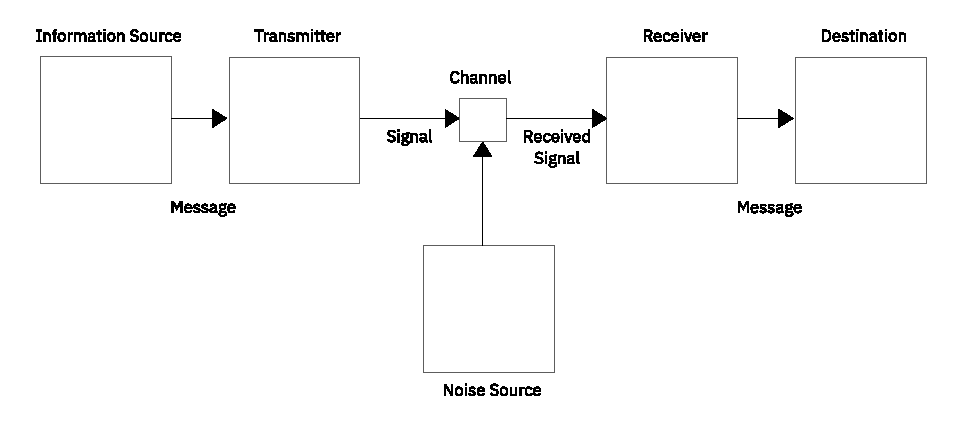
\includegraphics[width=\linewidth]{general-communication-system}
        \caption{Schematic diagram of a general communications system}
        \label{fig:gencomms}
    \end{figure*}

    In the case of digimorse, the information is a message in Morse code, the transmitter and receiver are a typical
    amateur radio transceiver and antenna system. The channel is therefore any of the amateur bands, typically using
    single-sideband (SSB) modulation. As will be seen in subsequent sections, digimorse is a \emph{narrow bandwidth}
    signal.

    In amateur radio, Morse code is traditionally transmitted using a single continuous radio wave, oscillating at a
    fixed frequency. This gives rise to the name and acronym it is more commonly known as: Continuous Wave, or CW.
    This method of transmitting Morse originated around 1913, with the invention of the vacuum tube electronic
    oscillator by Edwin Armstrong and Alexander Meissner\footnote{See Wikipedia, 'Continuous wave'}. Prior to this,
    Morse was transmitted using primitive \emph{spark gap} transmitters, which created much electromagnetic
    interference, and had wide bandwidth. They were outlawed in 1934. The bandwidth of a CW signal is very low,
    compared to the systems it replaced\cite{Amos}. Perhaps surprisingly, CW, as a method of transmitting Morse code
    using radio, has not changed significantly since then. In the intervening years, great improvements to receiver
    technology have been made: receiver sensitivity and selectivity have improved; filtering and digital signal
    processing techniques have been applied to try to reduce or remove the noise that plagues reception\footnote{Just
    in time to counteract the effects of the multitude of digital devices we have brought into our homes, creating an
    electromagnetic smog that most people are completely unaware of!}.

    However, despite these advances, noise and fading effects introduced by ionospheric reflection still impact our
    ability to receive and decode Morse, as received using CW signals.

\section{Digital Communications Systems}
    \newthought{digimorse attempts to be an upgrade to CW}.

    In a little more detail, the path through a digital communications system such as digimorse (or any modern
    digital radio mode for that matter) comprises several main elements.

    \begin{figure*}[h]
        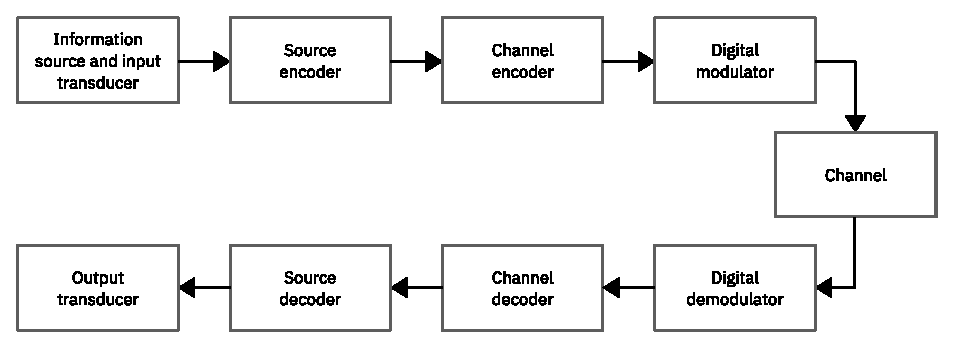
\includegraphics[width=\linewidth]{digital-communication-system}
        \caption{Basic elements of a digital communications system}
        \label{fig:digcomms}
    \end{figure*}


    \section{Project Website}

The website for the digimorse protocol and transceiver software is located at
\url{https://devzendo.github.io/digimorse}. On the website, you'll find
links to our \smallcaps{git} repository, mailing lists, bug tracker, and documentation.

\pagebreak
\appendix
\section*{Appendices}
\addcontentsline{toc}{section}{Appendices}
\renewcommand{\thesubsection}{\Alph{subsection}}

\subsection{Morse Code Speeds}

    \begin{table}[!h]
        \footnotesize
        \centering
        \fontfamily{ppl}\selectfont
        \begin{tabular}{llll}
            \toprule
            WPM & ms/dit & ms/dah & ms/wordgap \\
            \midrule
            5 & 240 & 720 & 1680 \\
            6 & 200 & 600 & 1400 \\
            7 & 171.4285714 & 514.2857143 & 1200 \\
            8 & 150 & 450 & 1050 \\
            9 & 133.3333333 & 400 & 933.3333333 \\
            10 & 120 & 360 & 840 \\
            11 & 109.0909091 & 327.2727273 & 763.6363636 \\
            12 & 100 & 300 & 700 \\
            13 & 92.30769231 & 276.9230769 & 646.1538462 \\
            14 & 85.71428571 & 257.1428571 & 600 \\
            15 & 80 & 240 & 560 \\
            16 & 75 & 225 & 525 \\
            17 & 70.58823529 & 211.7647059 & 494.1176471 \\
            18 & 66.66666667 & 200 & 466.6666667 \\
            19 & 63.15789474 & 189.4736842 & 442.1052632 \\
            20 & 60 & 180 & 420 \\
            21 & 57.14285714 & 171.4285714 & 400 \\
            22 & 54.54545455 & 163.6363636 & 381.8181818 \\
            23 & 52.17391304 & 156.5217391 & 365.2173913 \\
            24 & 50 & 150 & 350 \\
            25 & 48 & 144 & 336 \\
            26 & 46.15384615 & 138.4615385 & 323.0769231 \\
            27 & 44.44444444 & 133.3333333 & 311.1111111 \\
            28 & 42.85714286 & 128.5714286 & 300 \\
            29 & 41.37931034 & 124.137931 & 289.6551724 \\
            30 & 40 & 120 & 280 \\
            31 & 38.70967742 & 116.1290323 & 270.9677419 \\
            32 & 37.5 & 112.5 & 262.5 \\
            33 & 36.36363636 & 109.0909091 & 254.5454545 \\
            34 & 35.29411765 & 105.8823529 & 247.0588235 \\
            35 & 34.28571429 & 102.8571429 & 240 \\
            36 & 33.33333333 & 100 & 233.3333333 \\
            37 & 32.43243243 & 97.2972973 & 227.027027 \\
            38 & 31.57894737 & 94.73684211 & 221.0526316 \\
            39 & 30.76923077 & 92.30769231 & 215.3846154 \\
            40 & 30 & 90 & 210 \\
            41 & 29.26829268 & 87.80487805 & 204.8780488 \\
            42 & 28.57142857 & 85.71428571 & 200 \\
            43 & 27.90697674 & 83.72093023 & 195.3488372 \\
            44 & 27.27272727 & 81.81818182 & 190.9090909 \\
            45 & 26.66666667 & 80 & 186.6666667 \\
            46 & 26.08695652 & 78.26086957 & 182.6086957 \\
            47 & 25.53191489 & 76.59574468 & 178.7234043 \\
            48 & 25 & 75 & 175 \\
            49 & 24.48979592 & 73.46938776 & 171.4285714 \\
            50 & 24 & 72 & 168 \\
            51 & 23.52941176 & 70.58823529 & 164.7058824 \\
            52 & 23.07692308 & 69.23076923 & 161.5384615 \\
            53 & 22.64150943 & 67.9245283 & 158.490566 \\
            54 & 22.22222222 & 66.66666667 & 155.5555556 \\
            55 & 21.81818182 & 65.45454545 & 152.7272727 \\
            56 & 21.42857143 & 64.28571429 & 150 \\
            57 & 21.05263158 & 63.15789474 & 147.3684211 \\
            58 & 20.68965517 & 62.06896552 & 144.8275862 \\
            59 & 20.33898305 & 61.01694915 & 142.3728814 \\
            60 & 20 & 60 & 140 \\
            \bottomrule
        \end{tabular}
        \caption{Morse code speed in words per minute and the timing of the elements in milliseconds.}
        \label{tab:normaltab}
    \end{table}

\pagebreak
\bibliography{the-digimorse-communications-protocol}
\bibliographystyle{plainnat}



\end{document}
